\section{Question 2}
% 
\subsection{Assessment of Normality Through Q-Q Plot Analysis}
% 
\begin{lstlisting}[style=rstyle]
# clear the console area
cat("\014")
# clear the environment var area
rm(list = ls())
# set work directory
setwd("C:/Users/QianZ/Documents/Project/ISDS/personal-assignment-2/RCode")

# Import data using base R function
sugar_data <- read.csv("./data/Sugar.csv")

# Generate a Q-Q plot using base R functions
qqnorm(sugar_data$x)
qqline(sugar_data$x, col = "red")

\end{lstlisting}
% 
% 
% 
% 
% 
% 
\begin{figure}[H]
    \centering
    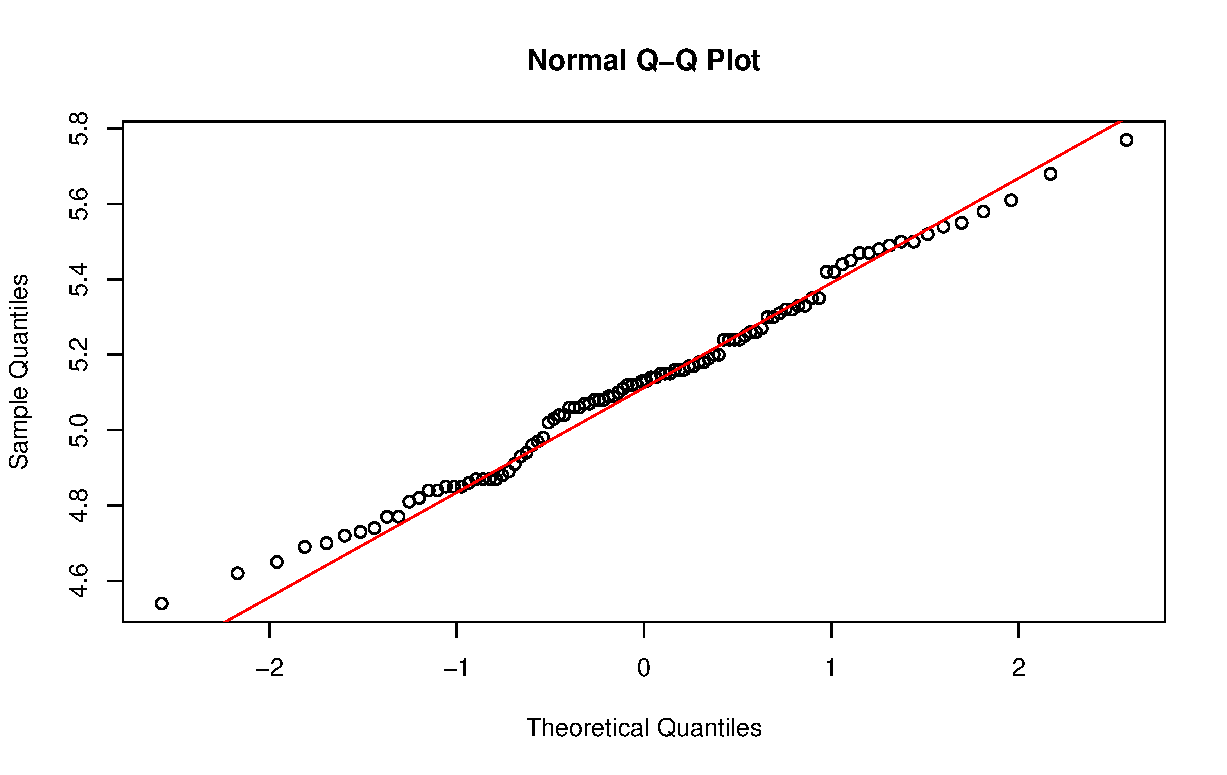
\includegraphics[width=\textwidth]{img/Q2_q1.pdf}
    \caption{The Q-Q plot of RStudio Output}
    % \label{fig:your-label}
\end{figure}
% 
% 
% 
% 
% 
% 
\paragraph{\textbf{Comments:} From the Q-Q plot (Figure 1), the data points are roughly arranged along the reference line, but there seems to be some deviation at both ends. This means that the data is approximately normally distributed in the central part, but there may be a slight bias in the tail.}
% 
% 
% 
% 
% 
% ----------------------------------------------------------------------------
% 
% 
% 
% 
\subsection{Shapiro-Wilks Test for Normality}
% 
% 
% 
% 
\begin{lstlisting}[style=rstyle]
# Perform the Shapiro-Wilk test on the sugar data
shapiro_test <- shapiro.test(sugar_data$x)

# Output the p-value from the test
shapiro_p_value <- shapiro_test$p.value

# Print the p-value
print(shapiro_p_value)

# Comment on the p-value
if (shapiro_p_value > 0.05) {
    cat("The p-value is greater than 0.05, suggesting that the null hypothesis of normality cannot be rejected.")
} else {
    cat("The p-value is less than or equal to 0.05, suggesting that the null hypothesis of normality can be rejected.")
}

\end{lstlisting}
% 
% 
% 
% 
% 
% 
% 
% 
% 
% 0.6553473
\paragraph{\textbf{Analytics:} The p-value is \textbf{0.6553473}, and output "The p-value is greater than 0.05, suggesting that the null hypothesis of normality cannot be rejected". This means that we do not have sufficient evidence to reject the null hypothesis of normal distribution, which is consistent with the observation in Q-Q plots that the data are mostly centered around the center, although the tail is slightly off.}
% 
% 
% 
% 
% 
% 
% 
% 
% 
\subsection{Two-Tailed Hypothesis Test for Sugar Amount}
% 
% 
% 
% 
% 
% 
\begin{itemize}
    \item Zero hypothesis ($h_0$): the average amount of sugar add equals 5 ml.
    \item Alternative hypothesis ($h_1$): the average amount of sugar add is not equal to 5 ml.
\end{itemize}
% 
% 
% 
% 
% 
\paragraph{The test statistic is calculated and the corresponding critical value is found. Since the sample size is less than 30, a t-distribution is used to determine the cut-off value.}
% 
% 
% 
% 
% 
$$ $$
% 
% 
% 
\begin{lstlisting}[style=rstyle]
# Define the significance level
alpha <- 0.05

# The null hypothesis (H0): The mean amount of sugar added is 5 ml
# The alternative hypothesis (H1): The mean amount of sugar added is not 5 ml

# Calculate the test statistic (t-value)
t_test <- t.test(sugar_data$x, mu = 5, alternative = "two.sided")

# Output the test statistic
t_value <- t_test$statistic

# Print the value of the test statistic
print(t_value)

# Find the critical t-value for a two-tailed test at the 5% significance level
critical_t_value <- qt(alpha/2, df=length(sugar_data$x)-1, lower.tail=FALSE)

# Print the critical t-value
print(critical_t_value)

# Conclusion based on the t-test
if (abs(t_value) > critical_t_value) {
    cat("Conclusion: Reject the null hypothesis. There is a significant difference between the amount of sugar I am adding and the 5 ml I am supposed to be adding.")
} else {
    cat("Conclusion: Fail to reject the null hypothesis. There is no significant difference between the amount of sugar I am adding and the 5 ml I am supposed to be adding.")
}
    
\end{lstlisting}
% 
% 
% 
% 
% 
% 
% 
% 
% 
\paragraph{\textbf{Conclusion:}}
% 
% 
% 
% 
% 
% 
% 
\begin{itemize}
    \item In the two-tailed hypothesis test, The test statistic (t-value) is \textbf{4.8981};
    \item on a t-distribution with 99 degrees of freedom, the critical t-value of the 5\% significance level is \textbf{1.984217} $\Rightarrow$ Because the absolute value of the test statistic is greater than the critical value, we can reject the null hypothesis.
    \item P-value is much smaller than the significance level $\alpha$ (0.05), which further supports the rejection of the null hypothesis.
\end{itemize}
% 
% 
% 
% 
% 
% 
% 